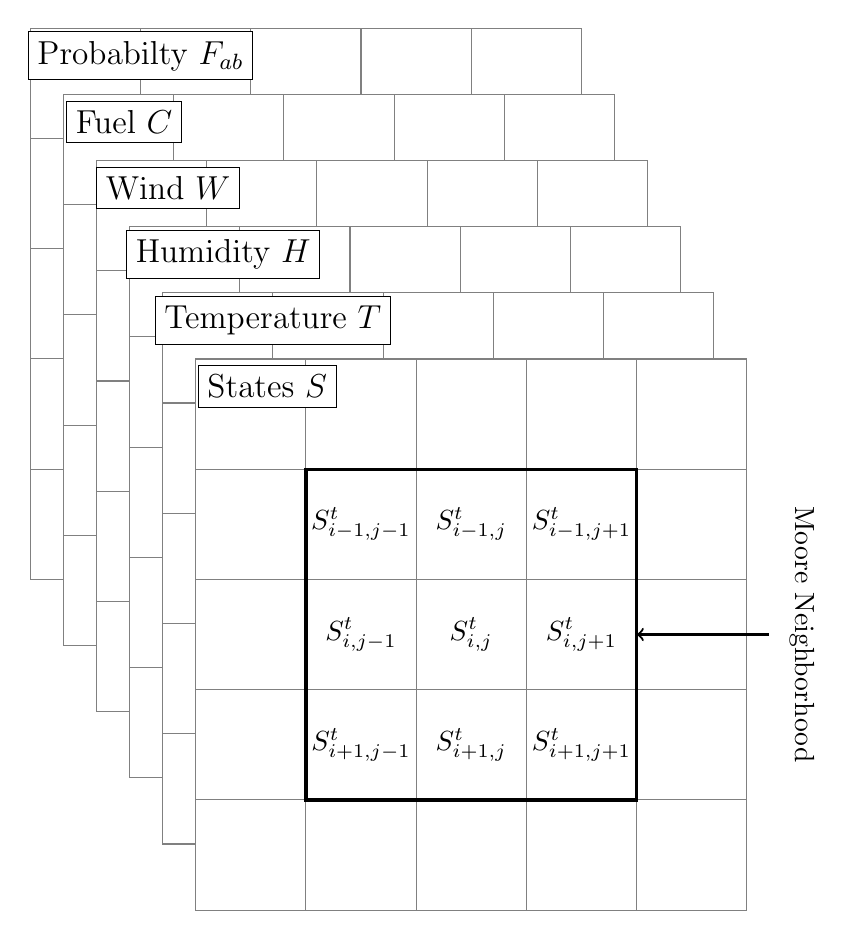
\begin{tikzpicture}[scale=1.4]
    
    \begin{scope}[xshift=-1.5cm, yshift=3cm]
        \draw[draw=gray, fill=white] (0, 0) grid (5, 5) rectangle (0,0); % grid
        \node[draw, fill=white] at (1, 4.75) {\large Probabilty $F_{ab}$}; % Layer name
    \end{scope}
    
    \begin{scope}[xshift=-1.2cm, yshift=2.4cm]
        \draw[draw=gray, fill=white] (0, 0) grid (5, 5) rectangle (0,0); % grid
        \node[draw, fill=white] at (.55, 4.75) {\large Fuel $C$}; % Layer name
    \end{scope}

    \begin{scope}[xshift=-.9cm, yshift=1.8cm]
        \draw[draw=gray, fill=white] (0, 0) grid (5, 5) rectangle (0,0); % grid
        \node[draw, fill=white] at (.65, 4.75) {\large Wind $W$}; % Layer name
    \end{scope}
    
    \begin{scope}[xshift=-.6cm, yshift=1.2cm]
        \draw[draw=gray, fill=white] (0, 0) grid (5, 5) rectangle (0,0); % grid
        \node[draw, fill=white] at (.85, 4.75) {\large Humidity $H$}; % Layer name
    \end{scope}
    
    \begin{scope}[xshift=-.3cm, yshift=.6cm]
        \draw[draw=gray, fill=white] (0, 0) grid (5, 5) rectangle (0,0); % grid
        \node[draw, fill=white] at (1, 4.75) {\large Temperature $T$}; % Layer name
    \end{scope}

    \begin{scope}
        \draw[draw=gray, fill=white] (0, 0) grid (5, 5) rectangle (0,0); % grid
        \draw[very thick] (1, 1) rectangle (4,4); % Moore neighborhood
        
        % States
        \node at (2.5, 2.5) {$S_{i,j}^t$};
        \node at (2.5, 3.5) {$S_{i-1,j}^t$};
        \node at (2.5, 1.5) {$S_{i+1,j}^t$};
        \node at (1.5, 2.5) {$S_{i,j-1}^t$};
        \node at (3.5, 2.5) {$S_{i,j+1}^t$};
        \node at (1.5, 3.5) {$S_{i-1,j-1}^t$};
        \node at (1.5, 1.5) {$S_{i+1,j-1}^t$};
        \node at (3.5, 3.5) {$S_{i-1,j+1}^t$};
        \node at (3.5, 1.5) {$S_{i+1,j+1}^t$};
        
        % Layer name
        \node[draw, fill=white] at (.65, 4.75) {\large States $S$};

        \node [rotate=-90] at (5.5, 2.5) {Moore Neighborhood};
        \draw[->, thick] (5.2, 2.5) -- (4, 2.5);
    \end{scope}
    
\end{tikzpicture}